\chapter{Introducere}\label{ch:1intro}

\section{Internet of things}
	Nivelul de evoluție la care a ajuns tehnologia în zilele noastre, dă naștere dorinței de a spori confortul vieții cotidiene prin creșterea gradului de interconectare al dispozitivelor inteligente.

	Scopul primordial al conceptului de Internet Of Things este de a face posibilă comunicarea între obiectele care prezintă utilitate în viața de zi cu zi. Acesta reprezintă o rețea vastă de dispozitive interconectate care sunt capabile să ia decizii fără intervenție din exterior. Prin intermediul senzorilor sunt preluate diverse date din mediul înconjurător, date care, în urma prelucrărilor, determină execuția anumitor acțiuni.

	Contrar așteptărilor, ideea de Internet of Things nu a apărut recent. Primul dispozitiv care implementa conceptul de IoT a fost lansat în anul 1982, fiind reprezentat de un tonomat de Coca-Cola care putea să trimită informații pe internet referitoare la numărul de doze disponibile si temperatura băuturilor \cite{cokeMachine}. În anul 1990, invenția lui John Romkey, toaster-ul controlat prin internet \cite{simoniot}, stârnește tot mai mult interesul asupra ideii de control de la distanță al dispozitivelor. În decursul anilor, tot mai multe firme producătoare de electronice au încercat să ofere clienților produse care pot transfera date prin intermediul internetutlui. De exemplu, în anii 2000, firma LG a produs un frigider care se putea conecta la internet prin WiFi \cite{simoniot}.

	Chiar dacă dispozitivele care au marcat debutul IoT nu oferă funcționalități mult prea utile, în ultimii ani s-a dovedit că transferul de date între dispozitive, fără a utiliza conductori electrici, poate fi folositor chiar și în domenii cheie. Astfel, medicina, armata, transporturile și imobiliarele sunt doar câteva exemple de domenii care au fost influențate de acest concept.  

	Medicina - se urmărește implementarea conceptului de monitorizare de la distanță, prin intermediul unor aparate care au rolul de a înregistra date legate de starea de sănătate a pacientului și de a le trimite într-o bază de date accesibilă de către personalul medical \cite{medical}.

	Armata - prezintă dispozitive de spionaj și de supreveghere de ultimă generație, toate acestea fiind posibile datorită ideii de Internet of Things \cite{army}.

	Industria transporturilor - în acest domeniu, IoT poate fi ilustrat prin transferul de date între un autovehicul și infrastructură, pietoni sau un alt autovehicul. Acest concept poarta denumirea de V2X, iar beneficiul major pe care îl poate aduce este reducerea considerabilă a numărului de accidente \cite{V2X}.   

	Imobiliare - în zilele noastre, se întâlnește din ce în ce mai des ideea de casă inteligentă. Aceasta se rezumă la faptul că, dispozitivele inteligente din casă comunică atât intre ele cât și cu electrocasnicele, reușind sa creeze un mediu cât mai confortabil pentru locuitori.

	Faptul că domeniul IoT prezintă o utilitate care nu poate fi neglijată, explică creșterea exponențială a numărului de dispozitive interconectate. Conform unei statistici publicate de către Arne Holst, conducătorul echipei de cercetare din cadrul companiei Statista, se aproximează ca în 2030 să se ajungă la un număr mai mare de 25.4 miliarde de dispozitive IoT \cite{increaseOfIot}.

\bigskip

\begin{figure}[H]
   	\centering
    	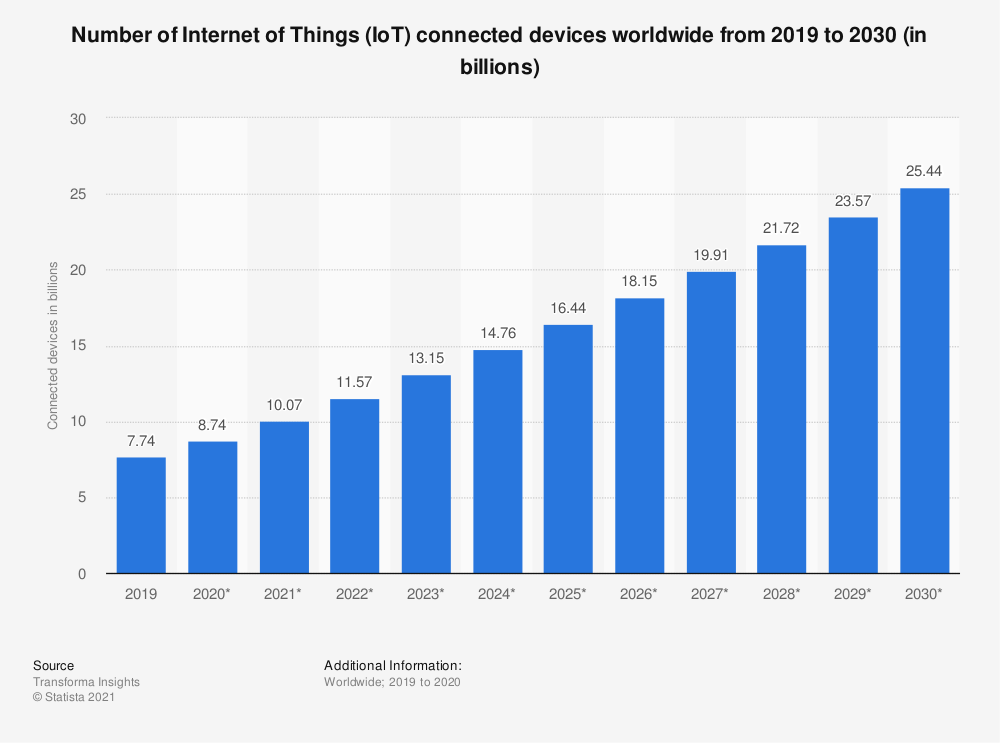
\includegraphics[width=0.8\textwidth]{Statistica-IoT.png}
	\caption{Evoluția numărului de dispozitive IoT (sursa: \cite{increaseOfIot})}
\end{figure}

\section{Contextul de realizare}\label{sec:context}
	Doresc ca prin intermediul proiectului să prezint beneficiile pe care automatizarea și conceptul de IoT le pot aduce. Sistemul creat abordează una dintre problemele care pot interveni la nivelul unei locuințe și se folosește de transferul de date la distanță, între diverse componente electronice, pentru a soluționa disconfortul termic.

	Problema pe care încerc să o rezolv, prin intermediul proiectului, am sesizat-o la apartamentul în care locuiesc. Acesta prezintă două camere de dimensiuni diferite, iar în sezonul rece ne confruntam cu un disconfort termic cauzat de diferențele de temperatură între cele două camere. Termostatul este montat în camera mare, fapt ce determina ca temperatura din camera mică sa fie mai mare decât cea setată. Nici mutarea termostatului in camera mică nu reprezenta o soluție, din cauză că timpul necesar încălzirii camerei mari este mai mare decât cel pentru camera mică, ajungându-se ca în camera mare sa fie tot timpul mai rece. Prin urmare, această inconveniență m-a motivat să creez un sistem care să reușească să mențină o temperatură constantă în apartament.

	La nivel non-tehnic, soluția constă în montarea în fiecare cameră a unor module ce monitorizează temperatura, iar în funcție de aceasta, comandă atât electrovalvele montate pe returul caloriferelor, cât și centrala. Rolul electrovalvei este de a închide sau deschide circuitul de apă din calorifer. De asemenea, este necesar ca lângă centrala termică să se monteze un modul care are rolul de a porni sau de a opri centrala în funcție de comanda primită de la modulele montate în camere. Acest modul se conectează la centrală prin intermediul unor fire, iar transferul de date între modulele din camere și modulul de control al centralei se face prin radio - frecvență. Pot fi setate temperaturi diferite pentru fiecare cameră în parte. Setarea se poate face fizic, prin intermediul unor butoane, sau de la distanță, prin intermediul unei aplicații web sau prin comenzi vocale interpretate de Google Assistant. Sistemul prezintă două moduri de funcționare. Primul mod constă în menținerea temperaturii setate, fără a ține cont de oră sau de faptul că ziua curentă este lucrătoare sau nu. Cel de-al doilea mod, oferă posibilitatea utilizatorului de a seta, prin intermediul aplicației web, temperaturi diferite pe anumite intervale orare ale zilei. Sistemul permite setarea a patru intervale orare în timpul zilelor lucrătoare ale săptămânii, iar pentru weekend pot fi setate două intervale.
